\documentclass[convert,float=true,crop=true]{standalone}
%\documentclass{article}
\usepackage{amssymb,amsmath}
\usepackage{hyperref}
%\url{https://tex.stackexchange.com/q/681708/86}
\usepackage[dvipsnames]{xcolor}
\usepackage{tikz}
\usetikzlibrary{
  tilings.polykite,
  calc,
  backgrounds
}

\begin{document}

\centering
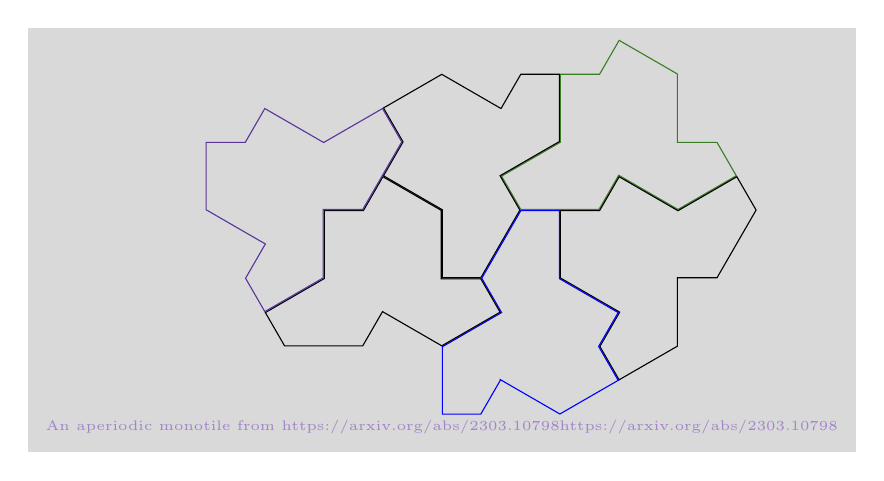
\begin{tikzpicture}[
  every aperiodical hat/.style={
    draw,
    thick
  },
  background rectangle/.style={fill=gray!30}, 
  show background rectangle
]
\pic[OliveGreen, aperiodical hat,name=hat-a];
\pic[aperiodical hat,name=hat-c,align with=hat-a along 13 using 6];
\pic[flip tile, aperiodical hat,name=hat-d,align with=hat-a along 26 using 2];
\pic[blue, aperiodical hat,name=hat-d,align with=hat-a along 24 using 3];
\pic[aperiodical hat,name=hat-e,align with=hat-d along 26 using 7];
\pic[RoyalPurple, flip tile, aperiodical hat,name=hat-f,align with=hat-e along 21 using 5];
\node[node font=\tiny] (A) at (-2.5,-3.625) [RoyalPurple!50] {An aperiodic monotile from \href{https://arxiv.org/abs/2303.10798}{https://arxiv.org/abs/2303.10798}};
\end{tikzpicture}
\end{document}
